\chapter{Sensoren}
Informatie over de buitenwereld krijg je door middel van sensoren. Sensoren zijn er in allerlei soorten en maten, maar werken vaak op hetzelfde principe. Een fysische gebeurtenis wordt geconverteerd naar een elektrisch signaal dat kan worden verwerkt door de microprocessor. Dit hoofdstuk bevat recepten voor het uitlezen van een aantal sensoren.

\newpage
\section{Potentiometer}
\paragraph{Probleem:} Je wilt een potentiometer uitlezen.
\paragraph{Benodigdheden:}
\begin{itemize}
	\item 1x Potentiometer
	\item 1x \SI{4.7}{\kilo\ohm} weerstand
\end{itemize}
\paragraph{Oplossing:}
\begin{figure}[H]
	\center{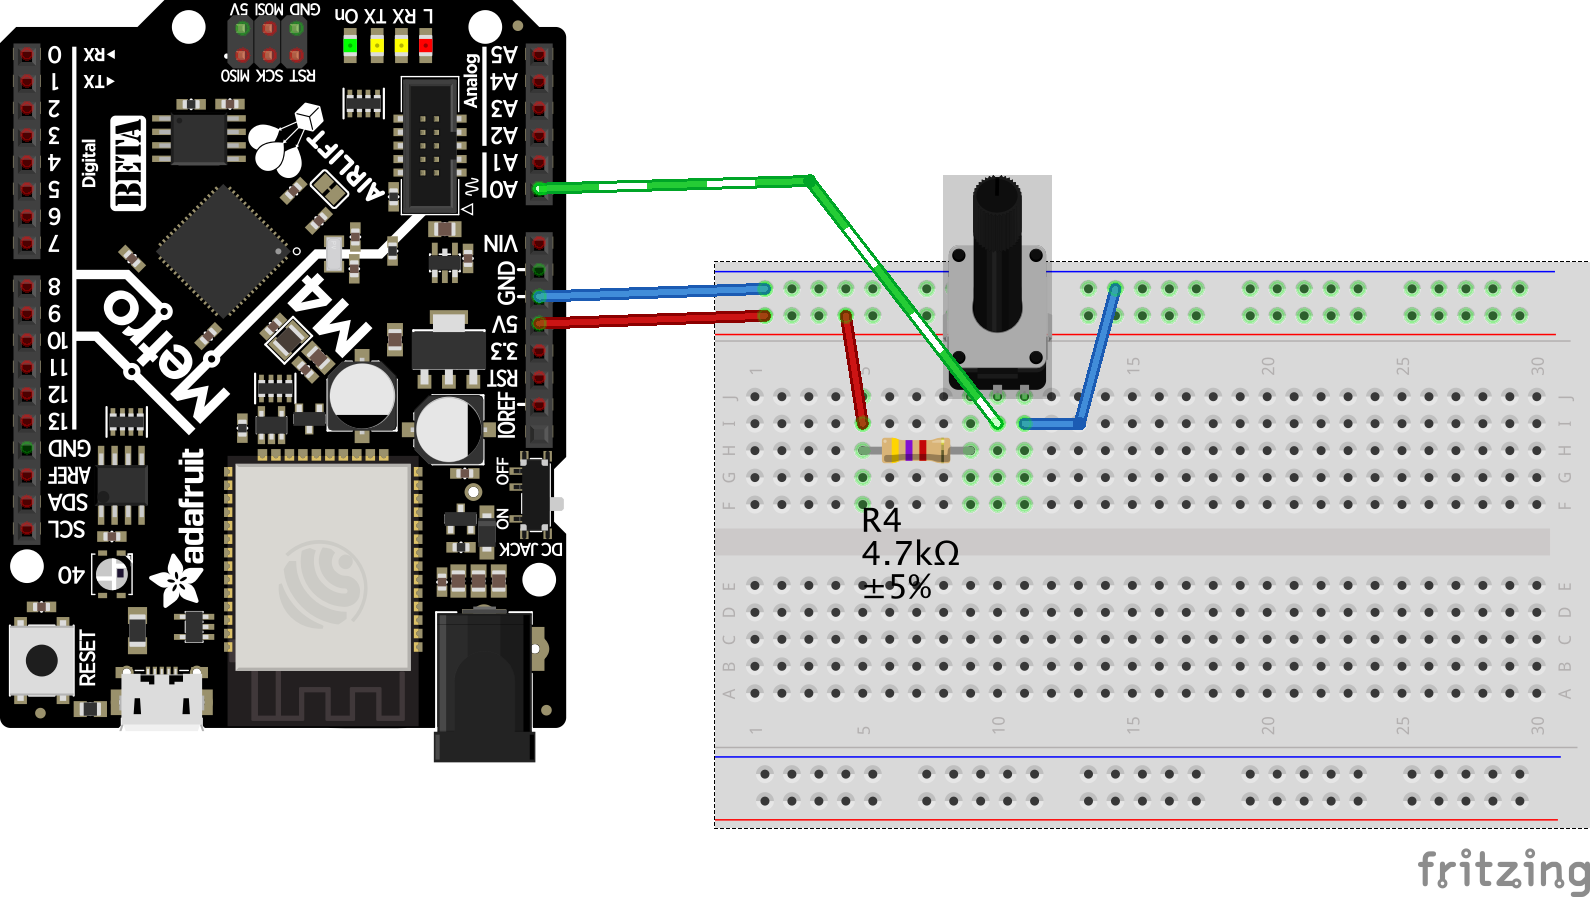
\includegraphics[width=\linewidth]{figures/PotSensor.png}}
	\caption{Potentiometer Sensor Circuit}
	\label{fig:PotSensor}
\end{figure}
\lstinputlisting{code/Lightsensor_TEMT6000.py}
\paragraph{Discussie:} Een potentiometer is een variabele spanningsdeler. Een potentiometer verbindt zowel de eerste pin en tweede pin met een weerstand als de tweede en derde pin met een weerstand. Door aan de potentiometer te draaien verander je de verhouding tussen de 2 weerstanden. Een potentiometer van \SI{10}{\kilo\ohm} heeft wel altijd een totale weerstand van \SI{10}{\kilo\ohm} tussen de eerste en derde pin. Door aan de pin te draaien kan je de verhouding wel veranderen in bijvoorbeeld \SI{1}{\kilo\ohm} tussen pin 1 en 2 en \SI{9}{\kilo\ohm} tussen pin 2 en 3 of \SI{0}{\kilo\ohm} tussen 1 en 2 en \SI{10}{\kilo\ohm} tussen 2 en 3.  Als \SI{3.3}{\volt} op pin 1 staat en pin 3 verbonden is met ground verandert de spanning op pin 2 evenredig meet de stand van de potentiometer. Omdat de tweede pin van de potentiometer in dit circuit direct zit aangesloten op een I/O pin, wordt een extra resistor toegevoegd om een short-circuit te voorkomen. Dit kan gebeuren in het geval dat de weerstand tussen pin 1 en pin 2 \SI{0}{\ohm} is.

Voor het uitlezen van een analoog signaal heeft CircuitPython de analogio bibliotheek. In de code hoef je alleen een object te maken door het analoge pin nummer als parameter aan de AnalogIn() functie te geven. De waarde van de spanning op de pin kan dan uitgelezen worden door objectnaam.value aan te roepen in de code.  De analoge waarde wordt uitgedrukt in een 16-bit digitaal getal. Een 16-bit digitaal getal kan 65536 waarden representeren, de waarden 0-65535. De waarde 0 wordt uitgelezen als een spanning van \SI{0}{\volt} op de pin wordt gezet en de waarde 65535 als een spanning van \SI{3.3}{\volt} op de pin wordt gezet. Om het digitale getal te converteren naar de analoge spanning wordt in de gedefinieerde get\_voltage() functie de uitgelezen waarde gedeeld door het aantal mogelijke nummers en vermenigvuldigd met 3.3. In de while loop wordt vervolgens elke tiende seconde de waarde geprint. Open ook de \textbf{plotter} in Mu editor om de waarden in de grafiek te zien veranderen als je aan de potmeter draait.

\newpage
\section{Een licht aan en uit zetten op basis van de licht intensitiet}
	\paragraph{Probleem:} Je wilt een automatisch licht dat aangaat als het donker wordt.
	\paragraph{Benodigdheden:}
	\begin{itemize}
		\item 1x LED
		\item 1x \SI{680}{\ohm} weerstand
		\item 1x TEMT6000 lichtsensor
	\end{itemize}
	\paragraph{Oplossing}:	
		\begin{figure}[H]
			\center{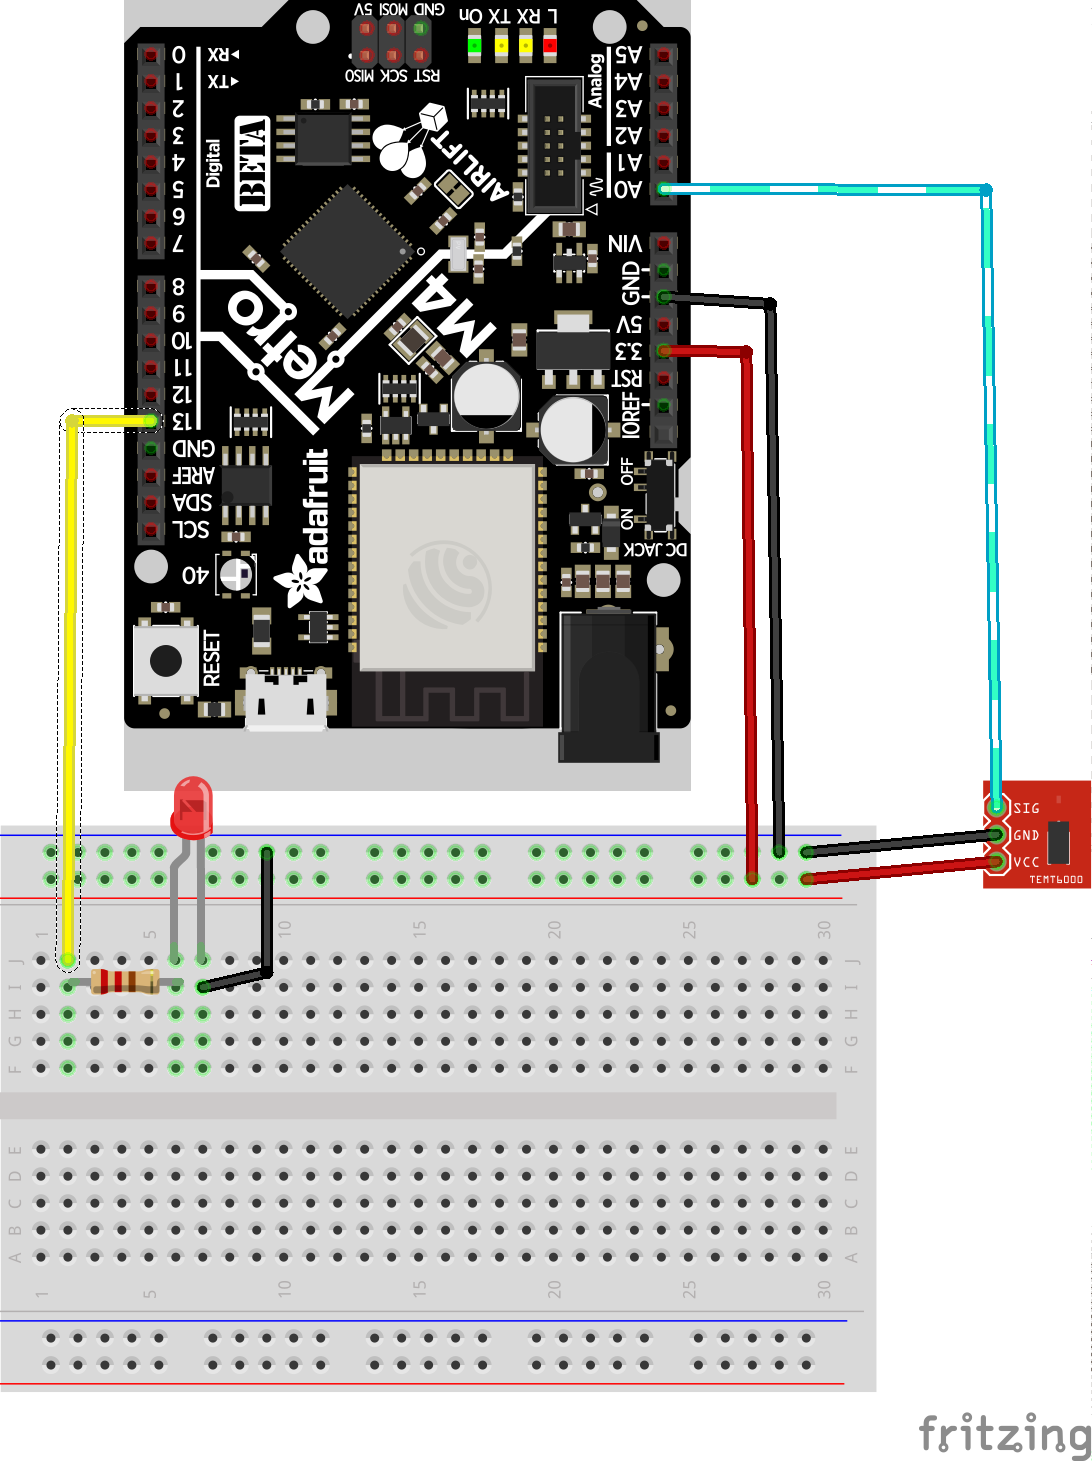
\includegraphics[width=0.6\linewidth]{figures/LightSensor_TEMT6000.png}}
			\caption{TEMT6000 lightsensor circuit}
			\label{fig:Lightsensor}
		\end{figure}
\newpage
		\lstinputlisting{code/Lightsensor_TEMT6000_OnOff.py}
	\paragraph{Discussie:} De lichtsensor is een analoge sensor waar een spanning uitkomt die evenredig is met de lichtintensiteit. De werking van een lichtsensor is vergelijkbaar met dat van een potentiometer, beide werken met het principe van een spanningsdeler. In het geval van een lichtsensor is het alleen niet een mechanische draaiknop dat de verhouding tussen de weerstanden verandert, maar de lichtintensiteit. De code om de spanning van de lichtsensor uit te lezen is precies hetzelfde als bij de potentiometer. De analogio module wordt ge\"importeerd en uitgelezen met de get\_voltage() functie. In dit geval wordt niet alleen de waarde van de sensor uitgelezen, maar wordt ook een LED aangezet als de lichtintensiteit een sensor spanning lager dan \SI{1.65}{\volt} geeft.
	

\newpage	
\section{Een licht feller laten branden als het donkerder wordt.}
    \paragraph{Probleem:} Je wilt de felheid van een ledje aanpassen op de intensiteit van het licht.
    \paragraph{Benodigdheden:}
    \begin{itemize}
    	\item 1x LED
    	\item 1x \SI{680}{\ohm} weerstand
    	\item 1x TEMT6000 lichtsensor
    \end{itemize}
    \paragraph{Oplossing:} Circuit in Figuur~\ref{fig:Lightsensor}
		\lstinputlisting{code/Lightsensor_TEMT6000_PWM.py}
	\paragraph{Discussie:}
		Dit is een variatie op het aan en uitzetten van de lichtsensor. Hier wordt \textbf{P}ulse-\textbf{W}idth \textbf{M}odulation gebruikt om het ledje feller en minder fel te maken op basis van de lichtintensiteit. De pulseio module wordt ge\"importeerd om PWM te gebruiken. In plaats van een DigitalInOut wordt nu een PWMout object gemaakt met de naam 'pwm' die geassocieerd is met pin D13. De intensiteit van de LED kan nu geregeld worden door de waarde pwm.duty\_cycle te veranderen. Ook PWM heeft een waarde tussen 0 en 65535, net als het uitlezen van een analoog signaal. De duty\_cycle is lineair gerelateerd aan het voltage uit de pin. Een waarde van 0 zet een spanning van 0V op de I/O pin en 65535 een waarde van 3.3V. In de code wordt een spanning van 3.3V op de pwm pin gezet als een lichtintensiteit van 0V wordt gemeten, 1.65V als 1.65V wordt gemeten en 0V als een spanning van 3.3V wordt gemeten.






\newpage
\section{Ultrasone afstandssensor}
	\paragraph{Probleem:} Je wilt de afstand tot een object meten met een ultrasone sensor.
	\paragraph{Benodigdheden:}
	\begin{itemize}
		\item 1x HCSR04 Ultrasone afstandssensor
	\end{itemize}
	\paragraph{Oplossing}:
	\begin{figure}[H]
		\center{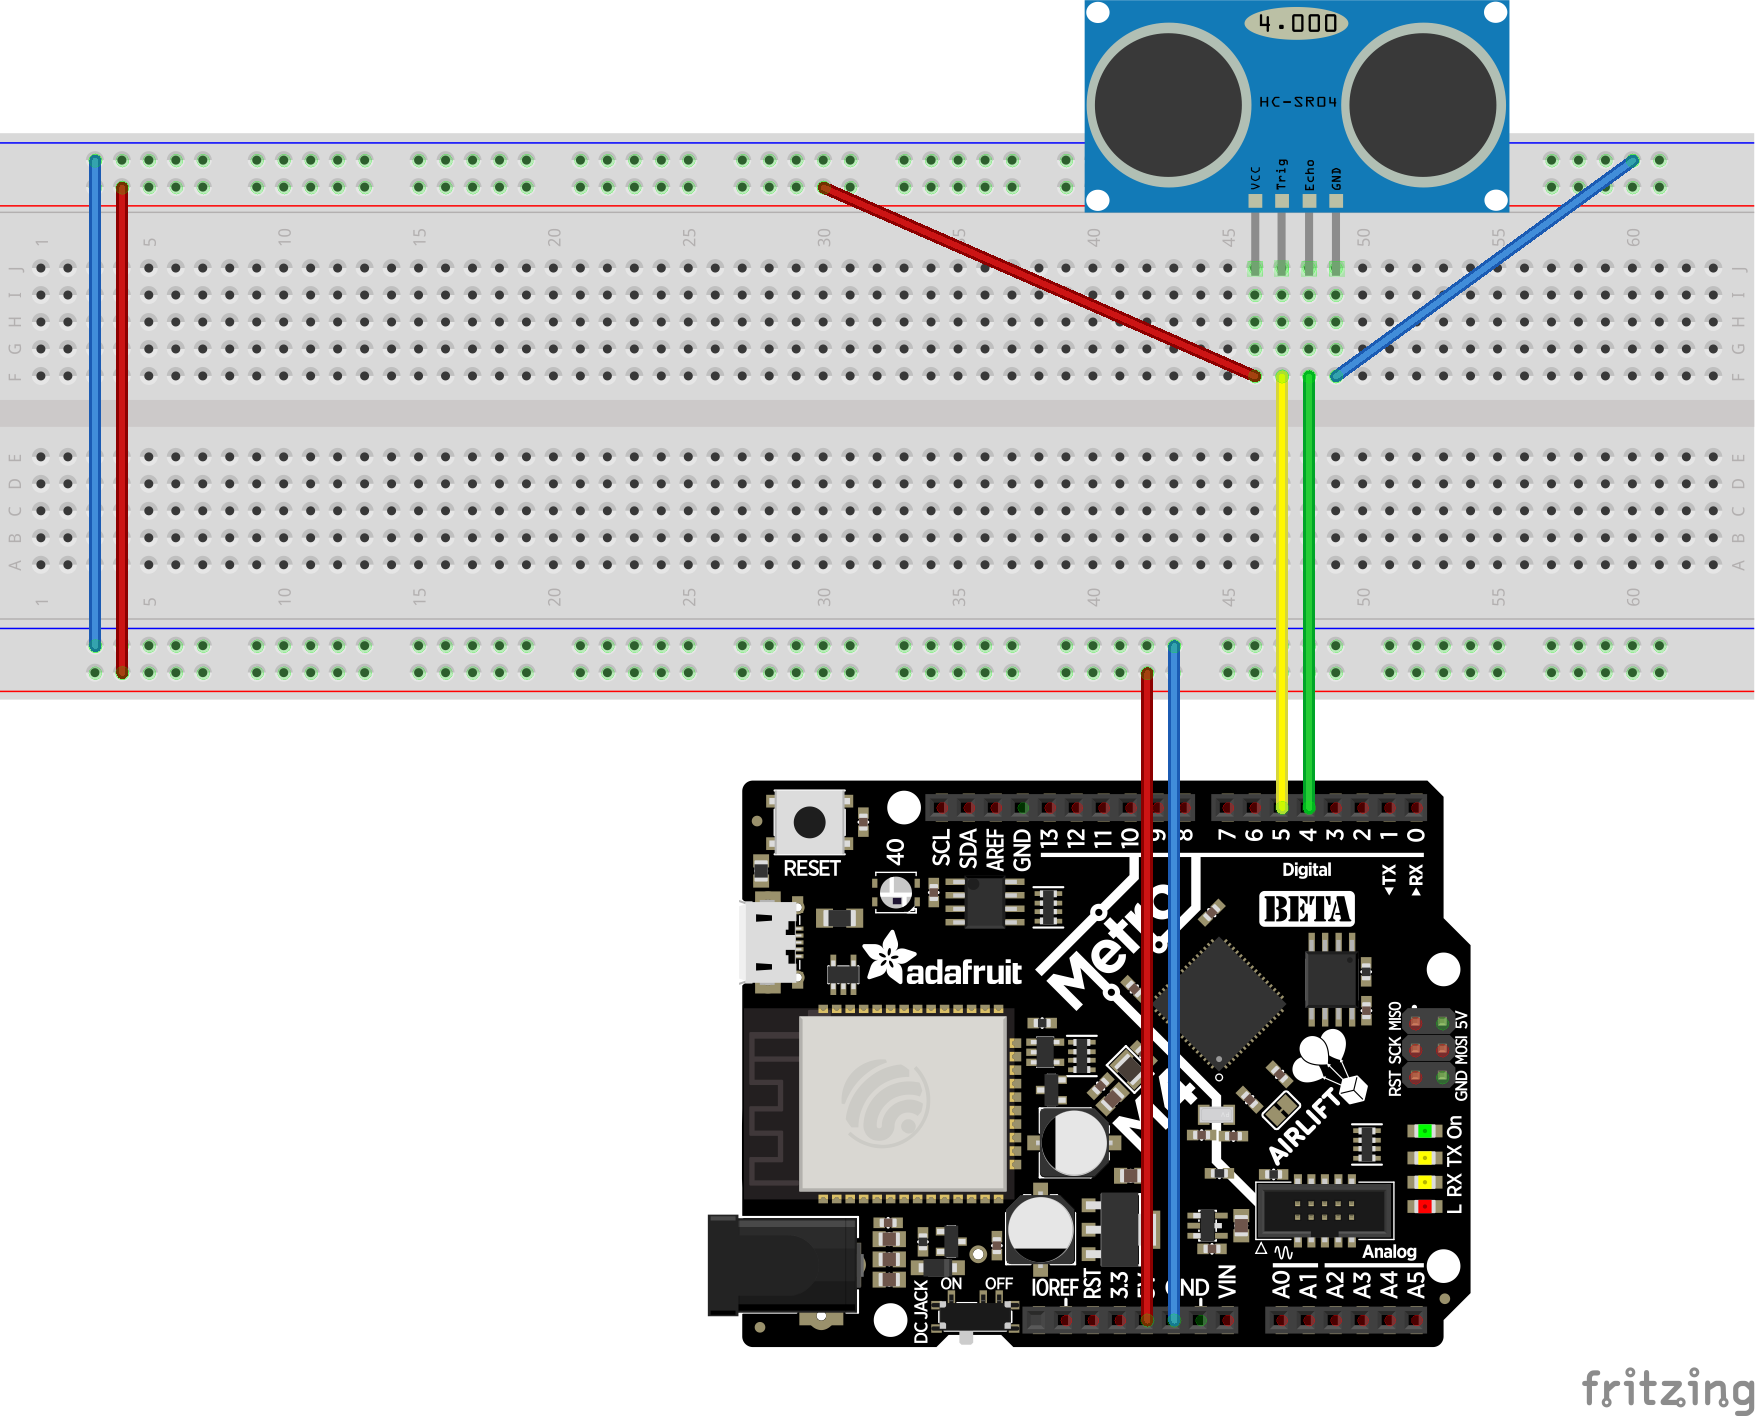
\includegraphics[width=0.6\linewidth]{figures/UltrasonicDistance.png}}
		\caption{Ultrasonic Distance Circuit}
		\label{fig:UltrasonicDistance}
	\end{figure}

%\newpage
	\lstinputlisting{code/UltrasonicDistance.py}
	\newpage
	
	\paragraph{Discussie:} Voor het gebruik van een ultrasone afstandssensor hoef je zelf weinig te programmeren, want Adafruit heeft hier een speciale bibliotheek voor in hun CircuitPython library bundel. Deze bundel kan je vinden op \url{https://circuitpython.org/libraries}. Zorg dat het adafruit\_hcsr04.mpy bestand in de lib folder op je bordje staat. 
	
	In de code hoef je nu alleen de adafruit\_hcsr04 te importeren en een nieuw object te maken met de HCSR04 functie, waarin je de trigger en echo pin nummers moet geven als parameters. Dit object krijgt in de code de naam sonar. De afstand kan nu eenvoudig gemeten worden door sonar.distance aan te roepen. Dit wordt in de code gedaan in een try/except block. Dit voorkomt dat de code crasht als er een runtime error optreedt bij het aanroepen van sonar.distance.
	
\newpage
\section{Joystick}
	\paragraph{Probleem:} Je wilt een joystick uitlezen en gebruiken in een project. 
	\paragraph{Benodigdheden:}
	\begin{itemize}
		\item 1x Joystick
	\end{itemize}
	\paragraph{Oplossing}:
		\begin{figure}[H]
			\center{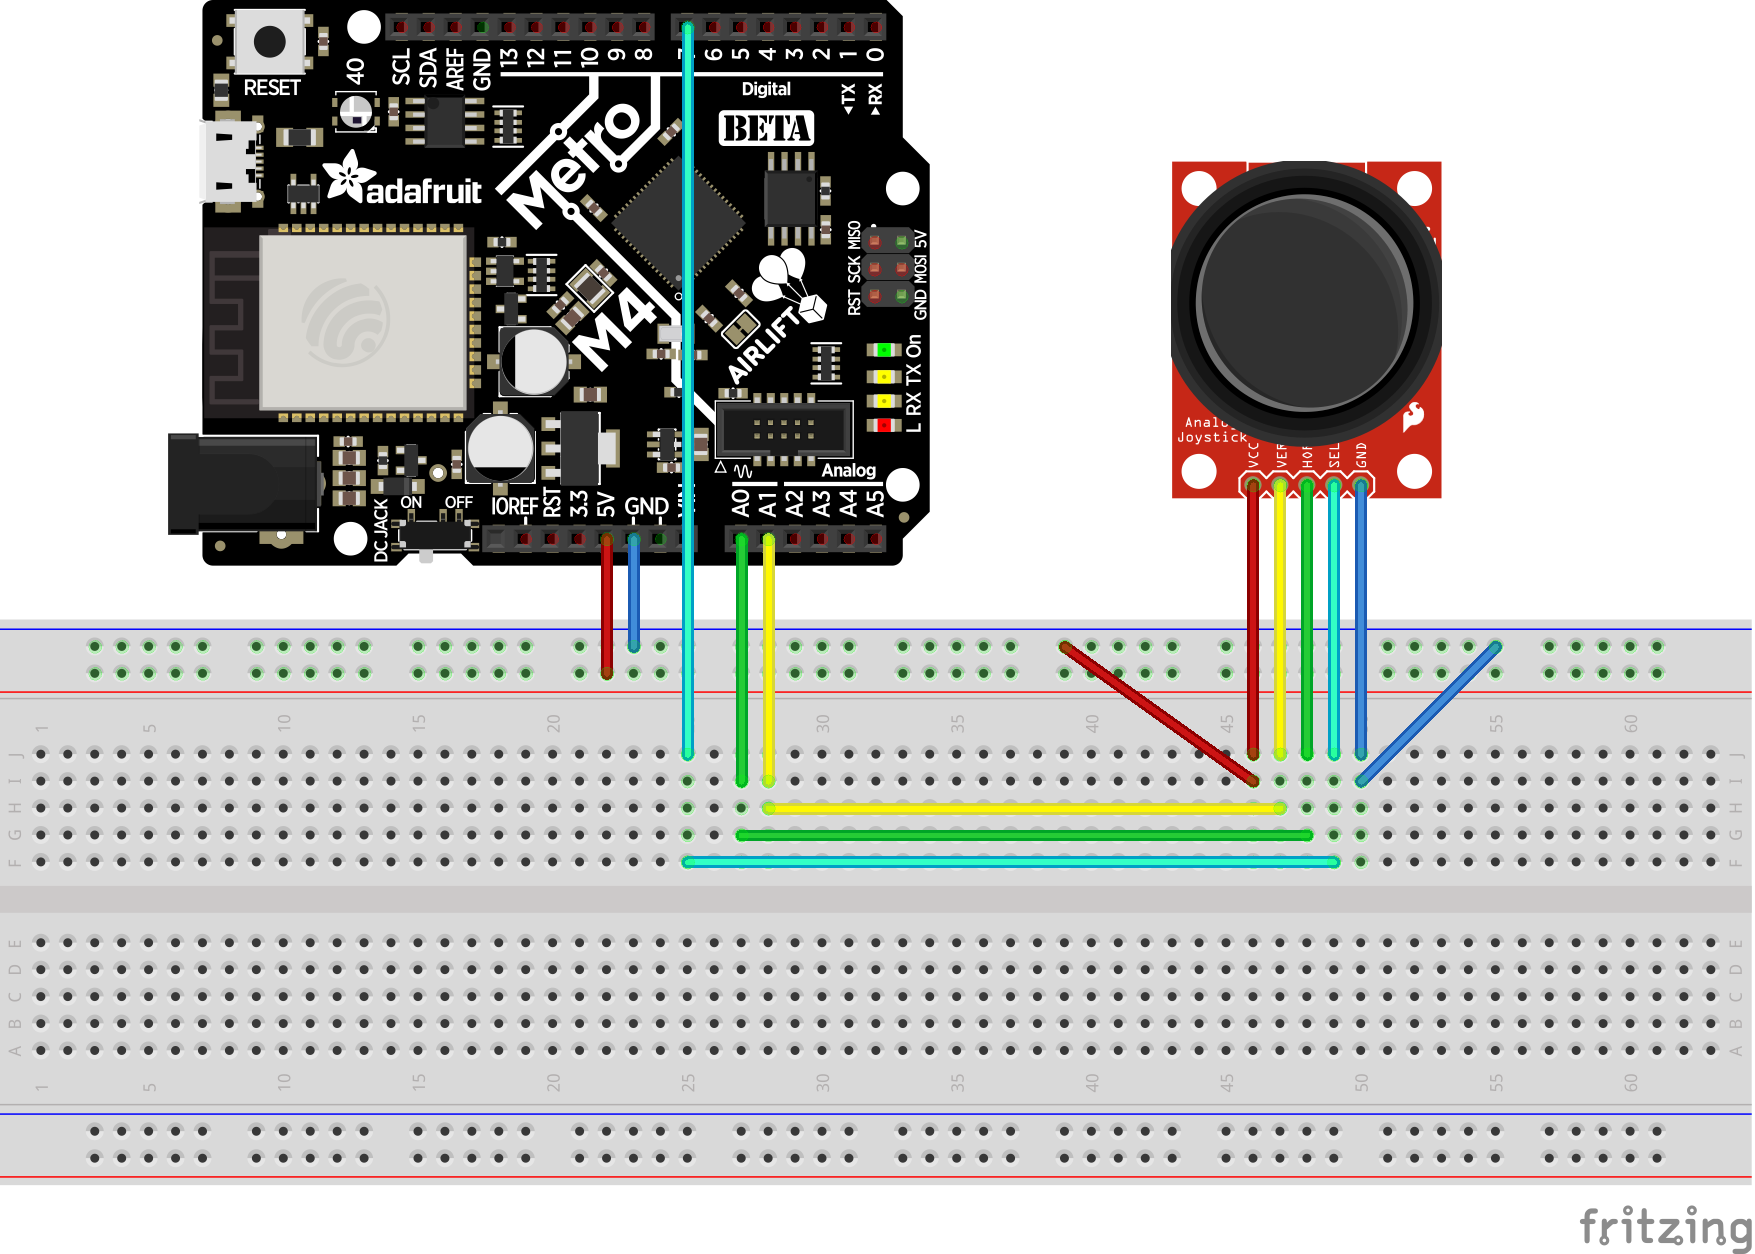
\includegraphics[width=0.8\linewidth]{figures/Joystick.png}}
			\caption{Joystick Circuit}
			\label{fig:Joystick}
		\end{figure}
	\newpage
		\lstinputlisting{code/Joystick.py}
	\paragraph{Discussie:} Een joystick bestaat uit 2 analoge potentiometers en 1 digitale knop. De benodigde modules voor het uitlezen van de joystick zijn de board, time, digitalio en analogio module.\\
	
	Links/rechts wordt uitgelezen op A1, omhoog/omlaag op A0 en het indrukken op D7.  De richting van D7 wordt op input gezet en een pull-up weerstand wordt gebruikt om de pin hoog te houden zolang de knop niet wordt ingedrukt. Als geen pull-up weerstand zou worden gebruikt, dan is niet bekend wat de waarde van de input is als de knop niet wordt ingedrukt. Het kan dan gebeuren dat de uitgelezen spanning dichter bij ground zit dan bij \SI{3.3}{\volt} en wordt dan uitgelezen alsof de knop wordt ingedrukt, terwijl dit niet gebeurd. Pull-up en pull-down weerstanden worden gebruikt om deze 'zwevende' waarden een vaste waarde te geven. \\
	
	In de oneindige while loop wordt elke tiende seconde eerst gekeken of de knop van de joystick is ingedrukt. Als dit niet zo is worden de 2 spanningen geprint. Als de knop wel wordt ingedrukt wordt "button pressed" geprint. Open ook de \textbf{plotter} in mu editor om de waarden te zien veranderen als je de joystick beweegt. 
	
	

\newpage
\section{RC Lowpass Filter}
	\paragraph{Probleem:} Je wilt het effect van een low-pass filter zien.
	\paragraph{Benodigdheden:}
	\begin{itemize}
		\item 1x \SI{15}{\kilo\ohm} weerstand
		\item 1x \SI{10}{\micro\farad} condensator
	\end{itemize}
	\paragraph{Oplossing}:
	\begin{figure}[H]
		\center{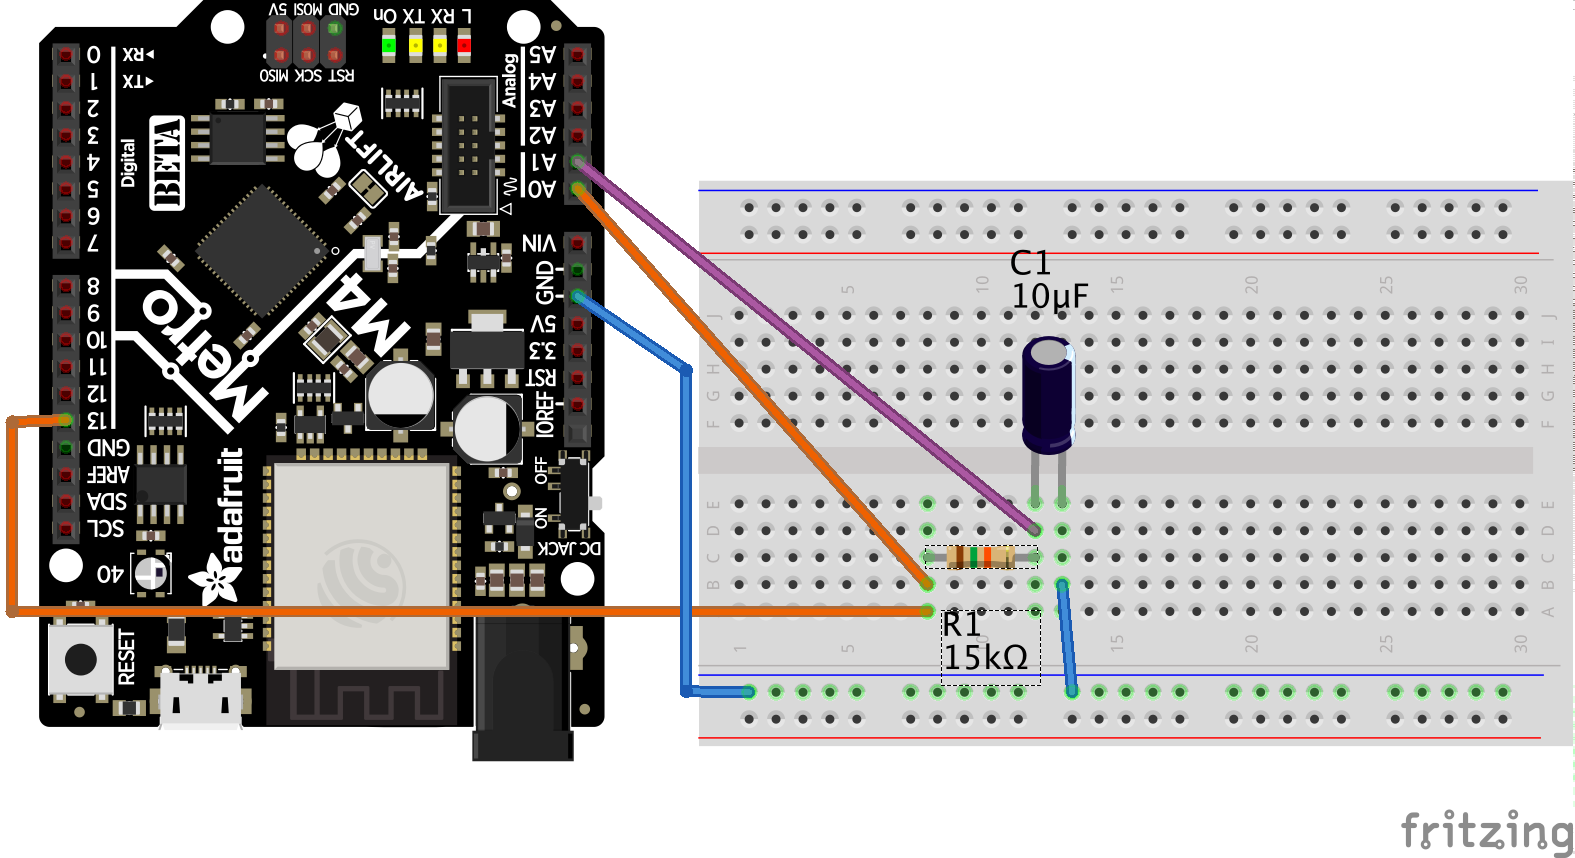
\includegraphics[width=0.8\linewidth]{figures/RC_Filter_PWM.png}}
		\caption{RC-filter Circuit}
		\label{fig:PWM_Filter}
	\end{figure}
	
	\newpage
	\lstinputlisting{code/PWM_Filter.py}
	\paragraph{Discussie:} Een \textbf{R}esistor \textbf{C}apacitor low-pass filter wordt gebruikt om hoge frequenties in signalen weg te filteren en lage frequenties door te laten. Low-pass filters worden vaak gebruikt om ruis uit sensor signalen te halen, maar ook door bijvoorbeeld dj's om hoge frequenties uit muziek te filteren. Om inzicht te krijgen in het effect van een RC-filter wordt in dit recept een PWM blokgolf gebruikt, die zowel gefilterd als ongefilterd wordt uitgelezen door een analoge input. \\
	
	De time, board, pulseio en analogio modules worden eerst ge\"importeerd. Er worden 2 analoge inputs ge\"initialiseerd op A0 en A1 en er wordt een PWM signaal  met een frequentie van 1 Hz en een duty cycle van 0.5 op pin D13 ge\"initaliseerd. \'E\'en signaal gaat direct van de PWM output naar A0. Dit signaal is ongefilterd. Het andere signaal gaat eerst door de RC filter voordat het bij A1 aankomt. De outputs worden vervolgens elke honderdste seconde geprint. Open de plotter in mu editor om de verschillende signalen te zien.
	
	